\chapter{Access Control I}
\label{chap:accessControl}
\thispagestyle{chapterInit}

\paragraph{Obbiettivi} Gli obbiettivi dei sistemi di controllo degli accessi sono:
    \begin{itemize}
        \item \textbf{Confidenzialità}: garantire che le informazioni siano accessibili solo a chi è autorizzato.
        \item \textbf{Integrità}: garantire che le informazioni non siano alterate da chi non è autorizzato.
    \end{itemize}

\section{\textit{Access Control}}
    \begin{figure}[H]
        \label{fig:accessControlSchema}
        \centering
        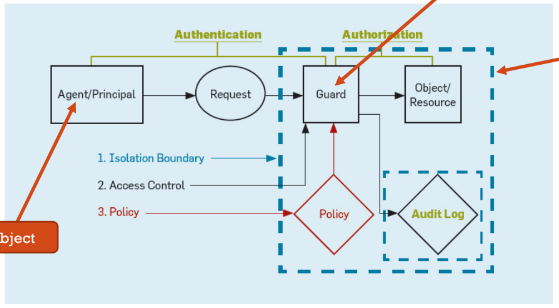
\includegraphics[scale=0.5]{06/AccessControSchema.png}
        \caption{Schema di un sistema di controllo degli accessi}
    \end{figure}

    Dallo schema raffigurato possiamo denotare che:
    \begin{itemize}
        \item \textbf{Soggetto} (\textit{Agent/Principal}): è l'entità che vuole accedere ad un oggetto o una risorsa, questo deve essere autenticato e autorizzato per poter accedere. Ad esempio un operatore di cassa di una banca non può accedere ai dati dei clienti, ma dopo aver ricevuto opportuna autorizzazione può effettuare operazioni sui conti.
        \item \textbf{Richiesta} (\textit{Request}): è la richiesta di accesso fatta dal soggetto. Questa contiene diverse informazioni che vedremo in seguito.
        \item \textbf{Confine di Isolamento} (\textit{Isolation Boundary}): è il confine che separa il soggetto dal sistema che contiene l'oggetto o la risorsa. Questo confine è importante per garantire che il soggetto non possa accedere direttamente all'oggetto o alla risorsa.
        \item \textit\textbf{Guard} (\textit{Policy Decision Point}): è l'entità che decide se il soggetto può accedere all'oggetto o alla risorsa. Questo prende decisioni basandosi su regole di autorizzazione.  
        \item \textit\textbf{Policy}: è l'insieme di regole che il \textit{guard} deve seguire per decidere se il soggetto può accedere all'oggetto o alla risorsa.
        \item \textbf{Oggetto} (\textit{Object/Resource}): è l'entità a cui il soggetto vuole accedere. Questo può essere un file, un database, un dispositivo, ecc\dots Questo deve essere protetto per garantire la confidenzialità e l'integrità delle informazioni.
        \item \textbf{Sistema Controllo Accessi} (\textit{Access Control }): è il punto dove avviene il controllo degli accessi. (Solitamente il \textit{guard} è una parte di questo sistema).
        \item \textit\textbf{Audit Log}: è il registro che contiene tutte le informazioni riguardanti le richieste di accesso sia autorizzate che non autorizzate. Questo è importante per monitorare il sistema e per rilevare eventuali attacchi.
    \end{itemize}
    
    \paragraph{Alcune note} Il confine di Isolamento tra il soggetto e tutto il resto del sistema è molto importante per garantire che nessuno possa accedere direttamente all'oggetto o alla risorsa senza passare per il \textit{guard}. Solo degli utenti con privilegi speciali, quali "amministratori" possono \textit{by-passare il guard} questo solo per aggiornare delle \textit{policy} o altri aggiornamenti al sistema. Infine è presente anche una \textit{inner boundary} che garantisce l'integrità dell'\textit{audit log}, questa non può essere \textit{by-passata} da nessuno, nemmeno dagli amministratori.
    \subsection{I Sistemi Operativi}
        I sistemi operativi sono esempi di sistemi che implementano il controllo degli accessi. Questi infatti non permettono di accedere direttamente alle risorse \textit{hardware} e \textit{software} del sistema, ma forniscono un'interfaccia per accedere a queste. Inoltre alcuni \texttt{SO} supportano multi-utente e multi-tasking, dove per il primo bisogna implementare un sistema per garantire accesso allo stesso tempo e/o in modo concorrente a più utenti, mentre per il secondo bisogna sviluppare un sistema per garantire che più processi in parallelo possano accedere alle risorse del sistema in modo concorrente.
        \subsubsection{Struttura del \texttt{SO}}
            Un sistema operativo è composto da una memoria, accessibile agli utenti, la quale comunica con il sistema operativo che tramite appositi meccanismi di controllo degli accessi permette di accedere al \texttt{I/O} \textit{bus} dove sono collocate le \texttt{I/O} \textit{interfaces} che permettono di accedere alle risorse del sistema (dischi, stampanti,\dots).\newline
            In questo sistema bisogna proteggere la memoria, i file contenuti nei dischi, controllare l'accesso degli utenti tramite meccanismi di autenticazione e autorizzazione e infine proteggere in generale il controllo degli accessi.
            \paragraph{Cosa implementa \texttt{SO}} Facendo riferimento alla figura \figref{fig:accessControlSchema}, il sistema operativo dunque implementa l'autenticazione, l'autorizzazione e la barriera di isolamento esterna per garantire che le \textit{policy} siano rispettate.
    \subsection{Definizione, Scopo e \textit{Policy} di un \texttt{AC}}
        \paragraph{Definizione} Un sistema di controllo accessi è definito come il processo che \textbf{media} le \textbf{richieste} alle risorse e ai dati di un sistema determinando se la richiesta di accesso deve essere approvata o rifiutata.
            \subparagraph{\textit{Flow} della richiesta} \begin{enumerate}
                \item Una richiesta di accesso $(s,a,r)$ viene fatta da un soggetto $s$ per accedere ad un oggetto $r$ tramite un'azione $a$. Questa arriva al modulo di controllo accessi
                \item Il modulo di controllo accessi prende la decisione se approvare (\textit{grant}) o rifiutare (\textit{deny}) la richiesta.
                \item Se la risposta è \textit{grant} allora $s$ può eseguire l'operazione $a$ su $r$, altrimenti se la risposta è \textit{deny} allora $s$ è informato che \underline{non} può eseguire l'operazione $a$ su $r$.
            \end{enumerate}
        Questo processo è di fondamentale importanza in un qualsiasi sistema di sicurezza.
    \subsection{Struttura di un \texttt{AC}}
        \paragraph{\textit{Policy}} La \textit{policy} sono le regole, ad alto livello, che controllano chi può accedere e che azioni possono eseguire su una particolare risorsa, o oggetto, che contiene informazioni.
        \paragraph{\textit{Model}} Il \textit{model} è la rappresentazione matematica formale della \textit{policy}, e come funziona una \textit{policy} in un sistema di controllo accessi.
        \paragraph{\textit{Enforcement}} L'\textit{enforcement} è l'\textit{hardware} o il \textit{software} che, a basso livello, implementano i controlli imposti dalle \textit{policy} e formalmente descritti nel \textit{model}.
        % Durante il corso è stato tralasciato la sezione "What can go wrong" 
\section{\textit{Access Control Models}}
    Il significato delle \textit{policy} si basa nella forma:
    \begin{quote}
        "Un soggetto $s$ può eseguire un'azione $x$ su un oggetto $o$
    \end{quote}
    una serie di queste affermazioni possono essere espresse nella forma di una matrice di controllo degli accessi (\textit{Access Control Matrix} \texttt{ACM}). Questa matrice è composta da righe e colonne, dove le righe rappresentano i soggetti (utenti) e le colonne rappresentano gli oggetti (risorse/files) e le celle contengono informazioni su chi è il proprietario dell'oggetto, chi può leggere o scrivere su di esso, ecc\dots
    \begin{table}[H]
        \centering
        \begin{tabular}{c|c|c|c|c|c|c|}
            \multicolumn{1}{c}{} & \multicolumn{1}{c}{\textit{f1}} & \multicolumn{1}{c}{\textit{f2}} & \multicolumn{1}{c}{\textit{f3}} & \multicolumn{1}{c}{\textit{f4}} & \multicolumn{1}{c}{\textit{f5}} & \multicolumn{1}{c}{\textit{f6}} \\
            \cline{2-7}
            \textit{s1} & &\textit{o, r, w} & \textit{o, r, w} &&& \\
            \cline{2-7}
            \textit{s2} & \textit{o, r, w} & \textit{r} & & & \textit{o, r, w} & \\
            \cline{2-7}
            \textit{s3} & & \textit{r} & \textit{r} & \textit{o, r, w} & \textit{r} & \textit{o, r, w} \\
            \cline{2-7}
        \end{tabular}
        \caption{Esempio di una \textit{Access Control Matrix}}
    \end{table}
    Altri sistemi di controllo accessi sono:
    \begin{itemize}
        \item \textit\textbf{Capability} (\texttt{C-list}): è un sistema dove ogni soggetto possiede una lista di capacità che gli permettono di accedere a determinate risorse. 
        \item \textit\textbf{Accesso Control List} (\texttt{ACL}): è un sistema dove ogni oggetto ha una lista di controllo degli accessi che contiene i soggetti che possono accedere all'oggetto e le azioni che possono eseguire.
    \end{itemize}
    Entrambe queste sono migliori della \texttt{ACM} in termini di efficienza, dato che non occupiamo spazio per le celle vuote ed sono molto più scalabili, il problema di tutte e tre è che bisogna verificare a monte se il richiedente è veramente chi dice di essere.

    \subsection{\texttt{ACL} v/s \texttt{C-list}}
        In questo genere di sistemi si usa come meccanismo di interazione con il sistema un \textit{compiler service} il quale si non può direttamente accedere e/o scrivere su un file, ma grazie ai permessi che eredita dagli utenti può farlo. Mentre il processi di lettura/scrittura avvengono viene aggiunta una riga ad un \textit{Bill file} il quale non può mai essere modificato direttamente da nessuno, ma solo dal \textit{compiler service} il quale vi scrive le informazioni necessarie per il controllo degli accessi.\newline
        Può accadere che il \textit{caller} confonda il \textit{compiler service} il quale restituisce il nome del \textit{billing file} al posto dell'oggetto richiesto in output, in questo caso l'integrità dell'\textit{Bill file} è compromessa e il sistema non è più sicuro.
        \subsubsection{\texttt{ACL}}
            Nel caso si usi un sistema \texttt{ACL} il problema risiede nel fatto che durante le operazioni il \textit{compiler service} è delegato dall'utente per l'accesso al file di output, e dal \texttt{SO} per l'accesso al \textit{billing file}. In quanto l'accesso avviene nella stesse esecuzione il \textit{compiler service} non può distinguere se l'accesso è stato fatto per conto dell'utente o del \texttt{SO}, quindi l'utente può scrivere sul \textit{billing file} e compromettere l'integrità del sistema.
        \subsubsection{\texttt{C-list}}
            Nel caso si usi un sistema \texttt{C-list} questo problema non si presenta in quanto l'utente non deve delegare esplicitamente l'accesso al file di input al \textit{compiler service} in quanto è il \texttt{SO} a farlo, quindi i permessi non vengono mai delegati dall'utente al \textit{compiler service}, ciò permette di evitare di confondere il \texttt{SO} con l'utente quando si scrive sul \textit{billing file}.
    \subsection{\textit{Confused Deputy in the cloud}}
        Il problema appena descritto si applica anche nel \textit{cloud}. Ad esempio se in un servizio si vuole delegare l'accesso a file o risorse ad altri account, questo è un esempio di accesso delegato. Nel cloud il problema di "\textit{confused deputy}" può accedere quando due utenti \texttt{A} e \texttt{B} ottengono il diritto all'esecuzione di un servizio \texttt{M}: Nel momento nel quale \texttt{A} viene concesso il diritto di scrittura viene inserita la coppia $(r,\texttt{M})$ nella \texttt{ACL} del servizio, quando ora \texttt{B} chiede di eseguire il servizio \texttt{M} per monitorare le risorse di \texttt{A} dato che \texttt{B} ha il diritto di eseguire il servizio \texttt{M} può leggere anche le risorse di \texttt{A}.\newline
        Per prevenire ciò bisogna implementare un \textbf{identificatore esterno} che deve essere univoco per ogni istanza del servizio \texttt{M}
    \subsection{Digressione sulla protezione nei sistemi operativi}
        Gli obbiettivi del \texttt{AC} per la protezione nei sistemi operativi sono:
        \begin{itemize}
            \item La prevenzione di uso malizioso delle risorse da parte degli utenti e/o processi.
            \item Il controllo che le risorse condivise siano usate secondo le \textit{policy} stabilite.
        \end{itemize}
        Per garantire ciò vengono stabiliti dei principi di protezione quali:
        \begin{description}
            \item[Principio del minimo privilegio] Un utente/processo deve avere solo i privilegi necessari per eseguire il suo compito. Questo garantisce che se un utente/processo è compromesso, il danno che può fare è limitato al suo ambiente e non può compromettere l'intero sistema.
            \item[Principio della conoscenza minimale] Un utente/processo deve avere accesso solo agli oggetti che deve conoscere per eseguire il suo compito. In questo modo si evita che un utente/processo possa accedere a risorse che non dovrebbe conoscere.
            \item[Dominio di protezione] Un dominio di protezione è una serie di oggetti e permessi che un utente/processo può eseguire su quegli oggetti. Formalmente un dominio di protezione è definito come segue: $$ \left< \texttt{object}, \{ \texttt{access rights} \} \right>$$ I domini di protezione possono essere implementati per utenti, processi o procedure. Un esempio di dominio di protezione è negli ambienti Unix/Linux dove ogni utente corrisponde ad un dominio di protezione.
        \end{description}
    \subsection{\texttt{AC} \textit{Models}}
        Esistono molti modelli di controllo degli accessi, i principali sono però:
        \begin{itemize}
            \item \texttt{DAC} (\textit{Discretionary Access Control}) I soggetti possono dare autorizzazione ad altri soggetti (\texttt{DISCRETIONARY})
            \item \texttt{MAC} (\textit{Mandatory Access Control}) Il sistema forza le regole di accesso (\texttt{MANDATORY})
        \end{itemize}
        \paragraph{\texttt{DAC}} I vantaggi in un modello \texttt{DAC} consistono principalmente nella flessibilità rispetto ad ogni singolo utente, inoltre la possibilità di delegare l'autorizzazione ad altri utenti rende questo sistema molto discrezionale, infatti il principale svantaggio è la difficoltà di gestire le autorizzazioni in un sistema con molti utenti da parte di un organo centrale, ciò significa che se ad esempio un utente non-it si dimentica di rimuovere un utente da una lista di controllo degli accessi, questo potrebbe avere accesso a risorse che non dovrebbe avere. Inoltre, se un utente è compromesso, allora tutte le risorse a cui ha accesso sono compromesse.
            \subparagraph{\texttt{DAC} \& gruppi} Nelle grandi organizzazioni è molto comune usare i gruppi per gestire le autorizzazioni, in quanto è molto più facile gestire i permessi di un gruppo piuttosto che di un singolo utente.
            \subparagraph{Attacchi \textit{trojan}} Un problema al quale i sistemi \texttt{DAC} sono soggetti è l'attacco \textit{trojan}, dove un utente malintenzionato (\textit{bob}) che normalmente non può accedere ad una risorsa ($r$) creando una risorsa $r'$ a cui può accedere e convincendo \textit{alice}, un utente autorizzato ad accedere alla risorsa originale $r$, a installare un programma \textit{trojan}, tramite tecniche di \textit{social engineering}, il quale legge il contenuto di $r$ e lo scrive su $r'$, in questo modo \textit{bob} può accedere alle informazioni di $r$.
        \paragraph{\texttt{MAC}} I vantaggi di un modello \texttt{MAC} sono che il sistema forza le regole di accesso, quindi non c'è bisogno di fidarsi degli utenti in quanto questi sono verificati e autorizzati da un organo centrale. Inoltre, se un utente è compromesso, solo le risorse a cui ha accesso sono compromesse, le altre risorse sono al sicuro. Gli svantaggi sono che il sistema è molto rigido e non flessibile, quindi per cambiare le autorizzazioni bisogna passare per un organo centrale, inoltre è molto difficile da implementare in sistemi con molti utenti.
            \subparagraph{Esempi di \textit{policy}} I permessi degli utenti vengono decisi dall'organizzazione che provvede anche a regolare come le risorse devono essere condivise. Ad esempio in un ospedale i dati dei pazienti non possono essere condivisi ed solo i medici che curano il paziente possono accedere ai dati del paziente. Viene introdotta anche una \textit{security label} che indica il livello di sicurezza, il personale che vi può accedere e l'orario di creazione della risorsa.
    \subsection{Sicurezza multi-livello}
        Le prime necessità nel garantire la sicurezza si sono verificate nel campo militare, dove diversi gradi di utenti possono accedere a diverse risorse, basate sul loro grado. Questo problema è nato ancora prima dell'avvento dei computer. Per garantire l'accesso a diversi livelli di risorse vengono effettuati dei controlli di sicurezza per evitare che utenti non autorizzati possano diffondere informazioni sensibili.
        \subsubsection{Implementazione}
            Per categorizzare le informazioni vengono introdotti dei livelli di \textit{sensitivity} in base a quanto quella risorsa è sensibile. Questi livelli vengono poi associati ad ogni risorsa in modo lineare all'importanza della risorsa. Esistono i livelli \textit{Top Secret} $\geq$ \textit{Secret} $\geq$ \textit{Confidential} $\geq$ \textit{Unclassified}. Questi livelli vengono poi associati ad ogni utente in base al loro grado, in modo che un utente con un grado più basso non possa accedere a risorse con un livello di sensibilità più alto.
        \subsubsection{Associazione dei livelli}
            Quando si crea una risorsa vi è associato il livello di \textit{sensitivity} e la corrispondente \textit{security label}, ciò avviene in base a criteri definiti in precedenza. Se in un documento sono presenti informazioni di livelli diversi allora il livello di sensibilità del documento sarà il livello più alto tra quelli presenti nel documento.\newline
            Esiste inoltre la possibilità che dopo qualche tempo il livello di sensibilità di una risorsa possa cambiare, in questo caso bisogna aggiornare la \textit{security label} della risorsa con il nuovo livello di sensibilità.
            \paragraph{Associazione agli utenti}
                Una volta che una risorsa è stata associata ad un livello di sensibilità, bisogna stabilire quali utenti sono autorizzati ad accedere a quella risorsa. Questo viene fatto associando ad ogni utente un livello di autorizzazione, che ha la stessa struttura di un livello di sensibilità. Un utente può accedere ad una risorsa se il suo livello di autorizzazione è maggiore o uguale al livello di sensibilità della risorsa. Formalmente una "\textit{clearance}" $C$ è composta da un livello di sicurezza gerarchico $S$ che indica il grado di affidabilità dell'utente ed un insieme di risorse "\textit{need-to-know}" $N$ che indica le risorse a cui l'utente deve poter accedere. ($C = (S,N)$)
        \subsubsection{Proprietà}
            Le proprietà di un sistema multi-livello sono:
            \begin{itemize}
                \item \textit\textbf{No read Up}: Un utente $s$ può leggere una risorsa $r$ se e solo se $(Ss,Ns)$ \textbf{domina} $(Sr,Nr)$ 
                \item \textit\textbf{No write Down}: Un utente $s$ può scrivere su una risorsa $r$ se e solo se $(Sr,Nr)$ \textbf{domina} $(Ss,Ns)$
            \end{itemize}
            Per \textbf{domina} intendiamo che $(S1,N1)$ domina $(S2,N2)$ se $S1 \geq S2$ e $N1 \supseteq N2$.\newline
            Anche se può sembrare contro-intuitivo il fatto che un utente con un livello di sensibilità più bassa possa scrivere su una risorsa con un livello di sensibilità più alto, questo è necessario non per garantire l'integrità della risorsa, ma per garantire la confidenzialità delle informazioni.
            % Multi-Level Security (6,7) SKIP
        \subsubsection{Pro e contro}
            I vantaggi di un sistema multi-livello sono che il sistema non è soggetto ad attacchi \textit{trojan} per la proprietà di \textit{no write down}, inoltre è rigido il che permette di tenere la situazione di controllo accessi sotto controllo, d'altra parte per cambiare le autorizzazioni bisogna passare per un organo centrale, inoltre il sistema è soggetto a \textit{information leakage by covert channels}, ovvero il passaggio di informazioni per mezzo di canali che nin sono stati progettati per trasmettere informazioni (eg. si è riuscito ad ottenere informazioni su quello che viene detto in una stanza analizzando il livello di luminosità della lampadina).
    \subsection{Ruolo / Gruppo / Utenti / Soggetti / Permessi / Sessioni - Definizioni}
        \subsubsection{Ruoli e Gruppi}
            Anche se i concetti di ruolo e gruppo possono sembrare simili, in realtà nella loro applicazione assumono un significato diverso. Formalmente:
            \begin{quote}
                Un \textit{ruolo} è un tipo di lavoro nel contesto di un'organizzazione, con della semantica associata, questa relativa le autorità e le responsibilità conferite al soggetto il quale ricopre quel ruolo.\texttt{[ANSI RBAC Standard]}
            \end{quote}
            Dunque i ruoli permettono di gestire i premessi in modo indiretto rispetto agli utenti, si può associare uno o più ruoli ad un utente e poi associare i permessi per eseguire una certa operazione a quel ruolo.\newline
            Un gruppo, molto più semplicemente, è un insieme di utenti.\newline
            Questo significa che ad un gruppo può essere associato un ruolo, ma ad un gruppo non può essere associato un permesso, questo in quanto i permessi non sono una cosa propria di un gruppo, ma di un ruolo.
        \subsubsection{Utenti e Soggetti}
            Spesso utente e soggetto vengono usati come sinonimi, nel nostro caso possiamo usarli come tali definendo:\newline
            Un utente è una persona fisica o un altro "\textit{active agent}" (programmi, applicazioni, \dots) che interagisce con il sistema. Ogni individuo deve essere conosciuto dal sistema come un solo utente (ecco perché l'autenticazione è un prerequisito per il controllo degli accessi)
            \paragraph{Associazione Utente-Ruolo (\texttt{UA})} Un utente può essere membro di uno o più ruoli. Un ruolo può avere uno o più membri.
            \paragraph{Associazione Ruolo-Permesso (\texttt{PA})} Un ruolo può avere uno o più permessi. Un permesso può essere associato a uno o più ruoli.
            \paragraph{Sessione} Un utente può invocare più sessioni, in ogni sessione un utente può invocare un sotto-insieme di ruoli dei quali è membro. Utile per garantire il principio del minimo privilegio.